\section{Protein synthesis}

Lastly, we turn our attention to the process of translation.  We begin by first
estimating the number of tRNA synthetases and ribosomes required to  double a
cell in 5000 seconds.  \textit{E. coli} has roughly 3 x 10$^6$ proteins per
cell, which for an average protein of 300 aa, amounts to the formation of
$\approx$ 10$^9$ peptide bonds. This value will also match the number of
amino-acyl tRNA that are required for protein synthesis, with the pool of tRNA continuously
recharging new amino acids by tRNA synthetases. At a rate of charging of about
20 amino-acyl tRNA per second (BNID: 105279, \cite{milo2010}), we find that
cells have more than sufficient tRNA synthetases to meet the ribosomal demand
(\FIG{protein_synthesis}(A)). If we consider an elongation rate of $\approx$ 15
peptide bonds per second (BNID: 114271, \cite{milo2010, dai2016}), the formation
of $\approx$ 10$^9$ peptide bonds would require about 1.5 x 10$^4$ ribosomes.
This is indeed consistent with the experimental data shown in
\FIG{protein_synthesis}(B).

\begin{figure}
    \begin{fullwidth}
    \centering{
        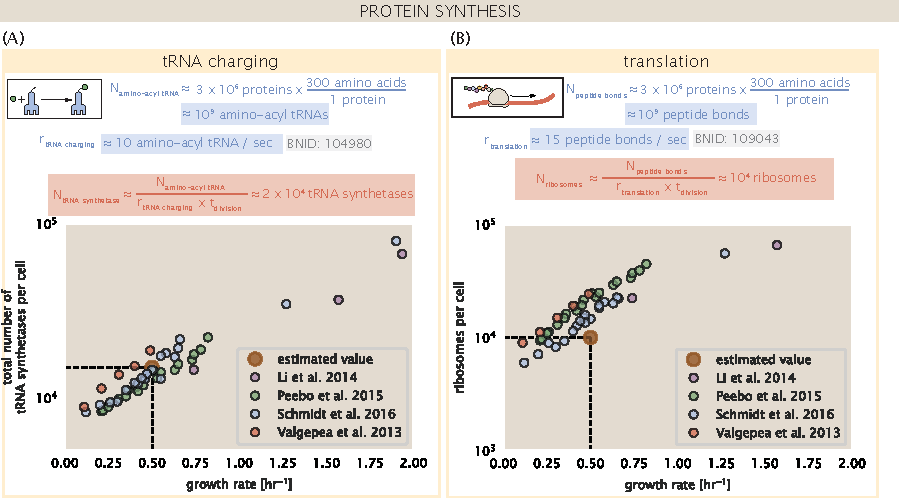
\includegraphics{main_figs/protein_synthesis.pdf}
        \caption{\textbf{Estimation of the required tRNA synthetases and
        ribosomes.} (A) Estimation for the
        number of tRNA synthetases that will supply the required amino acid
        demand. The sum of all tRNA synthetases copy numbers are plotted as a
        function of growth rate ([ArgS], [CysS], [GlnS], [GltX], [IleS], [LeuS],
        [ValS], [AlaS]$_2$, [AsnS]$_2$, [AspS]$_2$, [TyrS]$_2$, [TrpS]$_2$,
        [ThrS]$_2$, [SerS]$_2$, [ProS]$_2$, [PheS]$_2$[PheT]$_2$, [MetG]$_2$,
        [lysS]$_2$, [HisS]$_2$, [GlyS]$_2$[GlyQ]$_2$). (B) Estimation of the
        number of ribosomes required to synthesize 10$^9$ peptide bonds with an
        elongation rate of 15 peptide bonds per second. The
        average abundance of ribosomes is plotted as a function of growth rate.
        Our estimated values are shown for a growth rate of 0.5 hr$^{-1}$.}
    \label{fig:protein_synthesis}
    }
    \end{fullwidth}
\end{figure}

So far our estimates have led to protein copy numbers that are consistent with
the proteomic data, or even in excess of what might be needed for each task
under limiting growth conditions. Even in our example of \textit{E. coli} grown
under different carbohydrate sources (\FIG{carbon_tport}(B)), it becomes clear
cells can utilize alternative carbon sources by inducing the expression of
additional membrane transporters and enzymes. Optimal resource allocation and
the role of ribosomal proteins have been an area of intense quantitative study
over the last decade by Hwa and others \citep{scott2010, hui2015}. From the
perspective of limiting growth, our earlier estimate of rRNA highlighted the
necessity for multiple copies of rRNA genes in order to make enough rRNA. For
\textit{E. coli}'s fastest growth rates at 2 hr$^{-1}$, the additional  demand
for rRNA is further supported by parallelized DNA replication and increased rRNA
gene dosage. This suggests the possibility that synthesis of ribosomes might
be rate limiting. While the transcriptional demand for the ribosomal proteins
is substantially lower than rRNA genes, since proteins can be translated from
relatively fewer mRNA, other ribosomal proteins like the translation elongation
factor EF-Tu also present a substantial burden. For EF-Tu  in particular, it is
the most highly expressed protein in \textit{E. coli} and is expressed from
multiple gene copies, tufA and tufB.

To gain some intuition into how translation may set the speed limit for bacterial
growth, we again consider the total number of peptide bonds that must be synthesized,
$N_\text{AA}$. Noting that cell mass grows exponentially \citep{godin2010}, we
can compute the number of amino acids to be polymerized as \begin{equation}
N_\text{AA} = \frac{r_t R}{\lambda}, \end{equation} where $\lambda$ is the cell
growth rate in s$^{-1}$, $r_t$ is the maximum translation rate in amino acids
per second, and $R$ is the average ribosome copy number per cell. Knowing the
number of peptide bods to be formed permits us to compute the
translation-limited growth rate as \begin{equation}
\lambda_\text{translation-limited} = \frac{r_t R}{N_\text{AA}}.
\end{equation}

Alternatively, since $N_{AA}$ is related to the total protein mass through the
molecular weight of each protein, we can also consider the growth rate in terms
of the fraction of the total proteome mass that is dedicated to ribosomal
protein mass. By making the approximation that an average amino acid has a
molecular weight of 110 Da (see \FIG{translation_1}(A)), we can rewrite the
growth rate as,

\begin{equation}
\lambda_{\textrm{translation-limited}} \approx \frac{r_t}{L_R}  \Phi_R,
\label{eq:translation_limit_growth_rate}
\end{equation}
where $L_R$ is the total length in amino acids that make up a ribosome, and
$\Phi_R$ is the ribosomal mass fraction. This is plotted as a function of
ribosomal fraction $\Phi_R$ in \FIG{translation_1}(A), where we take $L_R
\approx$ 7500 aa, corresponding to the length in amino acids for all ribosomal
subunits of the 50S and 30S complex (BNID: 101175, \citep{milo2010}). This
formulation assumes that the cell can transcribe the required amount of rRNA,
which appears reasonable for \textit{E. coli}, allowing us to
consider the inherent limit on growth set by the ribosome.

The growth rate defined by Equation \ref{eq:translation_limit_growth_rate}
reflects mass-balance under steady-state growth and has long provided a
rationalization to the apparent linear increase in \textit{E. coli}'s
ribosomal content as a function of growth rate \citep{Goldberger1979,
scott2010}. For our purposes, there are several important consequences of
this trend. Firstly, we note there is a maximum growth rate of $\lambda
\approx 6 \text{hr}^{-1}$, or doubling time of about 7 minutes (dashed line).
This growth rate can be viewed as an inherent maximum growth rate due to the
need for the cell to double the cell's entire ribosomal mass. Interestingly,
this limit is independent of the absolute number of ribosomes and is simply
given by time to translate an entire ribosome, $L_R/ r_t$. As shown in
\FIG{translation_1}(B), we can reconcile this with the observation that in
order to double the average number of ribosomes, each ribosome must produce a
second ribosome. Unlike DNA replication or rRNA transcription, this is a
process that cannot be parallelized.

For reasonable values of $\Phi_R$, between about 0.1 - 0.3 \citep{scott2010},
the maximum growth rate is in line with experimentally reported growth rates
around 0.5 - 2 hr$^{-1}$.
% Here we are implicitly assuming that translation
% proceeds randomly, without preference between ribosomal or non-ribosomal mRNA,
% which appears reasonable.
Importantly, in order for a cell to scale this growth
limit they \textit{must} increase their ribosomal abundance.
This can be achieved by either synthesizing more ribosomes or reducing the
fraction of non-ribosomal proteins. Reduction of non-ribosomal proteins is not
a straightforward task since (as we have found throughout our estimates) doubling a
cell requires many other enzymes and transporters. Increasing the absolute
ribosomal abundance in \textit{E. coli} will be limited by the number of
rRNA operons.

\begin{figure}
  \begin{fullwidth}
        \centering{
            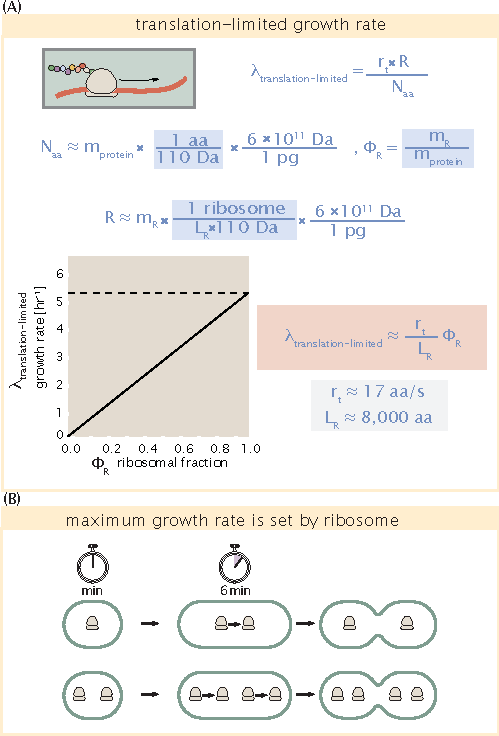
\includegraphics{main_figs/fig7_ribosome_growth_limit_3.pdf}
            \caption{\textbf{Translation-limited growth rate.} (A) Here we
            consider the translation-limited growth as a function of ribosomal
            fraction. By mass balance, the time required to double the entire
            proteome ($N_{AA}$ /$r_t$) sets the translation-limited
            growth rate, $\lambda_{\textrm{translation-limited}}$. Here $N_{aa}$
            is effectively the number of peptide bonds that must be translated,
            $r_t$ is the translation elongation rate, and $R$ is the number of
            ribosomes. This can also be re-written in terms of the ribosomal
            mass fraction $\Phi_R = m_R$ / $m_{\textrm{protein}}$, where $m_R$
            is the total ribosomal mass and $m_{\textrm{protein}}$ is the mass
            of all proteins in the cell. $L_R$ refers to the summed length of
            the ribosome in amino acids.
            $\lambda_{\textrm{translation-limited}}$ is plotted as a function of
            $\Phi_R$ (solid line). (B) The dashed line in part (A) identifies a
            maximum growth rate that is set by the ribosome. Specifically, this
            growth rate corresponds to the time required to  translation an
            entire ribosome, $L_R/ r_t$ . This is a result that is independent
            of the number of ribosomes in the cell as shown schematically here.
            }
        \label{fig:translation_1}
        }
  \end{fullwidth}
\end{figure}


\subsection{Multiple replication forks help bias ribosome abundance.}

\textit{E. coli} cells grow by a so-called "adder" mechanism, whereby cells add a constant
volume with each cell division \citep{taheriaraghi2015}. In conjunction with
this, additional rounds of DNA replication are triggered when cells reach a
critical volume per origin of replication (\FIG{translation_ecoli}(A)). This
leads to the classically-described exponential increase in cell size with growth
rate \cite{schaechter1958, si2017, si2019}. However, the mechanism behind growth rate
control has remained elusive and has only been described at a phenomenological level. In the context of maximizing growth rate,
it is notable that the majority of ribosomal proteins and rRNA operons are found
closer to the DNA origin. Given that cells must increase their total gene dosage
of rRNA operons at faster growth rates, and the intimate relationship between
ribosomal content and growth rate considered above, this raises the possibility
that the increase in chromosomal content might simply be a means for the cell
to tune biosynthesis according to its physiological state and the nutrient
availability in its environment.

While an increase in transcription has been observed for genes closer to the
origin in rapidly growing \textit{E. coli} \citep{scholz2019}, we were
unaware of such characterization at the proteomic level. In order to see
whether there is a relative increase in protein expression for genes closer
to the origin at faster growth, we calculated a running boxcar average (500
kbp window) of protein copy number as a function of each gene's
transcriptional start site (\FIG{translation_ecoli}(B)). While absolute
protein copy numbers can vary substantially across the chromosome, we indeed
observe a bias in expression under fast growth conditions (dark blue), showing the
result. The dramatic change in protein copy number near the origin is primarily
due to the increase in ribosomal protein expression. This trend is in
contrast to slower growth conditions (yellow) where the average copy number is more
uniform across the length of the chromosome.

\begin{figure*}
    \begin{fullwidth}
    \centering{
        \includegraphics{main_figs/fig8_ribosome_growth_limit_ecoli_3.pdf}
        \caption{\textbf{Multiple replication forks skew gene dosage and
        ribosomal content.} (A) Schematic shows the expected
        increase in replication forks (or number of ori regions) as \textit{E. coli} cells
        grow faster. (B) A running boxcar average of protein copy number is calculated for
        each each growth condition considered by
        Schmidt \textit{et al.}. A 0.5 Mb averaging window was used. Protein
        copy numbers are reported relative to their condition-specific means in order to center all
        data sets.
        (C) and (E) show experimental data from Si \textit{et al.} (2017)
        Solid lines show fits to the data, which were used to estimate
        $\langle$\# ori$\rangle$ / $\langle$\# ter$\rangle$ and $\langle$\# ori$\rangle$
        [NB: to note fit equations]. Red data points correspond to measurements in strain
        MG1655, while light green points are for strain NCM3722. (D) Plot compares our estimate of
        $\langle$\# ori$\rangle$ / $\langle$\# ter$\rangle$  to the experimental
        measurements of ribosomal abundance. Ribosomal fraction was approximated from
        the RNA/protein ratios of Dai \textit{et al.} (2016) (yellow) and Si \textit{et al.} (2017) (light red and light green) by the conversion RNA/protein ratio $\approx \Phi_R \cdot 2.1$.
        (F) Plot of the ribosome copy number estimated from the proteomic data against
         the estimated $\langle$\# ori$\rangle$.
        (G) Schematic showing translation-specific requirements for maintenance
        of steady-state growth. In a nutrient rich environment, amino acid supply $r_{aa}$ is sufficiently in
        excess of the demand by ribosomes translating at their maximal rate. In poorer
        nutrient conditions, reduced amino acid supply $r_{aa}$ will decrease
        the rate of elongation. In a regime where $r_{aa}$ is less than $r_t \cdot R$,
        the number of actively translating ribosomes will need to be reduced in order
        to maintain steady-state growth.
        (H) Translation elongation rate is plotted as a function of the number of actively translating ribosomes $R \cdot f_a$. Dashed lines correspond to a range of amino acid
        synthesis rates $r_{aa}$, from 10$^3$ to 10$^6$. Growth rates are calculated according to Equation 1, assuming a constant ribosomal fraction of 8 percent. See appendix XX for additional details.
        (I) Experimental data from Dai \textit{et al.} are
        used to estimate the fraction of actively translating ribosomes. The
        solid line represents the translation-limited growth rate for ribosomes
        elongating at 17.1 AA/s. }
        \label{fig:translation_ecoli}
    }
    \end{fullwidth}
\end{figure*}

If ribosomal genes (rRNA and ribosomal proteins) are being synthesized at
their maximal rate according to the rRNA gene dosage, we can make two related
hypotheses about how their ribosome abundance should vary with chromosomal
content. First, the ribosomal protein fraction should increase in proportion
to the average ratio of DNA origins to DNA termini ($\langle$\# ori$\rangle$
/ $\langle$\# ter$\rangle$ ratio). This is a consequence of the skew in DNA
dosage as cells grow faster. The second hypothesis is that the absolute
number of ribosomes should increase with the number of DNA origins
($\langle$\# ori$\rangle$), since this will reflect the total gene dosage at
a particular growth condition.

In order to test each of these expectations we considered the experimental data
from \cite{si2017}, which inferred these parameters for cells under
nutrient-limited growth. The ratio $\langle$\# ori$\rangle$ / $\langle$\#
ter$\rangle$ depends on how quickly chromosomes are replicated relative the
cell's doubling time $\tau$ and is given by 2$^{\tau_C / \tau}$. Here $\tau_C$
is the time taken to replicate \textit{E. coli}'s chromosome, referred to as the
C period of cell division.  In \FIG{translation_ecoli}(C) we plot the measured
$\tau_C$ versus $\tau$ (computed as $\tau = \log (2) / \lambda$), with data
points in red corresponding to \textit{E. coli} strain MG1655, and blue to
strain NCM3722. \cite{si2017} also measured the total RNA to protein ratio
which reflects ribosomal abundance and we show that data along with other recent
measurements from \cite{dai2016,dai2018}. Indeed, we find that the ribosomal
fraction increases with $\langle$\# ori$\rangle$ / $\langle$\# ter$\rangle$
(\FIG{translation_ecoli}(C)). We note a systematic difference in the relative
abundances from \cite{peebo2015} and \cite{valgepea2013} that was inconsistent
with a number of other measurements of total RNA-to-protein ratios ($\approx
\Phi_R$ x 2.1 \cite{dai2016}) and only show the data from \cite{schmidt2016} and
\cite{li2014} for relative ribosome abundances (see supplemental section XX for
a more complete discussion). For the data shown, the ribosomal fraction doesn't
increase as much at higher $\langle$\# ori$\rangle$ / $\langle$\# ter$\rangle$.
Since several rRNA operons are actually located approximately half-way between
the origin and terminus, the trend may in part be a consequence of a diminishing
increase in rRNA gene dosage at higher $\langle$\# ori$\rangle$ / $\langle$\#
ter$\rangle$ ratios.

We can similarly estimate $\langle$\# ori$\rangle$, which depends on how often
replication forks are initiated per cell cycle. This is given by the number of
overlapping cell cycles,  2$^{\tau_{cyc} / \tau}$, where $\tau_{cyc}$, refers to
the total time of chromosome replication and cell division.
\FIG{translation_ecoli}(E) shows the associated data from \cite{si2019},
which we use to estimate $\langle$\# ori$\rangle$  for each growth condition of
the proteomic data. In agreement with our expectations, we find that ribosome
copy number increases with the estimated $\langle$\# ori$\rangle$
(\FIG{translation_ecoli}(F)).

While it is difficult to distinguish between causality and correlation, the data
is at least consistent with the need for cells to increase their effective rRNA
gene dosage in order to grow according to the constraint set by Equation 2.
These results may also shed some light on the notable increase in ribosomal
content that is observed when sublethal doses of antibiotics \citep{scott2010,
dai2016}. Specifically, if rRNA synthesis is rate limiting, and nutrient
conditions largely dictate the extent of overlapping DNA replication cycles,
than addition of antibiotic will lengthen the doubling time and allow an
increased rRNA synthesis relative to the rate
of cell division. In Supplemental Section XX, we consider this further using
additional data from \cite{si2017}.

\subsection{Regulation of translating ribosomes helps maintain maximal growth
according to nutrient availability.}

While the above analysis provides a possible explanation for how \textit{E. coli}
can vary its ribosomal content to maximize growth, it also presents a
challenge in the limit of poorer nutrient conditions. Recall from Equation
\ref{eq:translation_limit_growth_rate} that ribosomal content should decrease to
zero as growth decreases to zero. While bacteria tend to decrease their
ribosomal abundance in poorer nutrient conditions, they do so only to some
fixed, non-zero amount \citep{scott2010, liebermeister2014}. Here we find a
minimal ribosomal fraction of $\approx$ 0.06 in the slowest growth conditions.
From the perspective of a bacterium dealing with uncertain nutrient conditions,
there is likely a benefit for the cell to maintain some relative fraction of
ribosomes to support rapid growth as nutrient conditions improve.

The challenge however, lies in the cell's ability to maintain steady-state
growth when ribosomes are in excess of the rate that nutrients can be harvested
and amino  acids synthesized for consumption \FIG{translation_ecoli}{G}. One
explanation for this is that the elongation rate decreases in poorer growth
conditions. Cells, however, are still able to maintain a relatively high
elongation rate even in stationary phase ($\approx$ 8 AA/s, \citep{dai2016,
dai2018}). A second explanation is that there are mechanisms to regulate
biological activity in conditions of stress and nutrient-limitation; in
particular through the small-molecule alarmones (p)ppGpp \citep{harris2018}.
Here we explore these two observations to better understand their consequence on
growth rate.

We consider slow growth conditions ($\lambda$ less than ~ 0.5 $hr^{-1}$) by
assuming that the decrease in elongation rate is due to a
limiting supply of amino acids and a need for the cell to maintain excess
nutrients for cellular homeostasis under steady-state growth. There is some
experimental support showing that in poorer nutrient growth conditions, cells
have lower amino acids concentrations  \citep{bennett2009}. We proceed by coarse
graining the cell's amino acid supply as an single, effective rate-limiting
species (see Supplmental Section XX for a more complete discussion). Under such a scenario,
the elongation rate can described as simply depending on the maximum elongation
rate ($\approx$ 17.1 aa/s, \citep{dai2016, dai2018}), an effective $K_d$, and
the limiting amino acid concentration $[AA]_{eff}$. Specifically, the elongation
rate is given by,

\begin{equation}
r_t = r_t^{max} \cdot \frac{1}{1 + K_d / [AA]_{eff}}.
\label{eq:rate_Kd}
\end{equation}
For cells growing in minimal media + glucose, the amino acid concentration is of
order 100 mM  (BNID: 110093, \citep{milo2010, bennett2009}). With a growth rate
of about 0.6 hr$^{-1}$ and elongation rate of 12.5 aa per second
\citep{dai2016}, we can estimate an effective $K_d$ of about 40 mM. Ultimately
the steady state amino acid concentration will depend on the difference between
the supply of amino acids $r_{aa}$ and consumption by ribosomes $r_t \cdot R
\cdot f_a$, where $f_a$ accounts for the possible reduction of actively
translating ribosomes.

In \FIG{translation_ecoli}{E} we consider how the maximal growth rate and
elongation rates vary as a function of the number of actively translating
ribosomes in this slow growth regime (see Supplemental Section XX for a complete
description of the model). If we consider $r_{AA}$ to be reflective of a specific
growth condition, by considering lines of constant $r_{AA}$, we find that cells
grow fastest by maximizing their fraction of actively translating ribosomes.
When we consider the experimental measurements from \cite{dai2018}, we see
that although cells indeed reduce $R \times f_a$, they do so in a way that keeps
$[AA]_{eff}$ relatively constant. Given our estimate for the $K_d$ of 40 mM,  we
would only expect a decrease from 100 mM to about 35 mM in the slowest growth
conditions. While experimental data is limited, amino acid concentrations only
decrease to about 60 mM for cells grown in minimal media + acetate ($\lambda$ ~
0.3 hr$^{-1}$ in our proteomic data; value obtained from \cite{bennett2009}), qualitatively consistent with our expectations.

Given the quantitative data from \cite{dai2018}, which determined $f_a$
across the entire range of growth rates across our data, we next estimated the
active fraction of ribosomal protein. As shown in \FIG{translation_ecoli}(G), we
find that cells grow at a rate near the expected translation maximum expected
from Equation 1, using the maximum elongation rate of $r_t$ = 17.1 aa per
second. This is in contrast to the reality that ribosomes are translating at
almost half this rate in the poorest growth conditions. This highlights that
there are alternative ways to grow according to the translated-limited growth
rate that is expected based with ribosomes translating at their maximal
elongation rate. Specifically, it is by adjusting $r_t \times R \times f_a
\approx r_{tmax} \times R'$ that cells are able to scale the growth limit set by
Equation 2.

[NB, These observations will be very important to include in
discussion section: A number of recent papers highlight the possibility that
(p)ppGpp may even provide a causal explanation for the nutrient-limit scaling
law. In the context of ribosomal activity, increased levels of (p)ppGpp are
associated with lower ribsomal content, and at slow growth appear to help reduce
the fraction of actively translating ribosomes \citep{dai2016, dai2018}.
Titration of the cellular (p)ppGpp concetrations (up or down) can invoke similar
proteomic changes reminiscent of those observed under nutrient limitation
\citep{zhu2019}. In light of the limiting dependence of ribosome copy number on
chromosomal gene dosage, it was recently shown that growth in a (p)ppGpp  null
strain abolishes both the scaling in cell size  and the $\langle$\# ori$\rangle$
/ $\langle$\# ter$\rangle$ ratio. Instead, cells exhibited a high $\langle$\#
ori$\rangle$ / $\langle$\# ter$\rangle$ closer to 4 and cell size more
consistent with a fast growth state where (p)ppGpp levels are low
\citep{fernandezcoll2020}.]



% [NB: to incorporate. Titration of the cellular ppGpp concetration invoked similar proteomic changes
% to those observed under nutrient limitation \citep{zhu2019}. In light of our
% hypothesis that such changes to the proteome are intimately linked to  the
% details of DNA replication, it was recently shown that both the  $\langle$\#
% ori$\rangle$ / $\langle$\# ter$\rangle$ and cell size lost their growth rate
% dependent scaling in a ppGpp null strain. Rather, cells exhibit a $\langle$\#
% ori$\rangle$ / $\langle$\# ter$\rangle$ closer to 4 and cell size more
% consistent with a fast growth state \citep{fernandezcoll2020}. This supports the
% possibility that in addition  to coordinating ribosome activity, (p)ppGpp
% signaling may be acting to coordinate other  cellular processes in accordance
% with nutrient conditions and biosynthetic demand. From this  perspective, the
% increase in the rate of DNA initation and associated increase in cell  size may
% be viewed as a way for the cell to vary its proteomic composition and
% biosynthetic  capacity according to its available nutrient conditions. ]

% In addition,
% given their massive size at about 850 kDa, they may play an as-yet fully
% understood role as a crowding agent in cellular function \cite{delarue2018,
% solerbistue2020}.

% [NB: to do. 1) slow growth regime, 2) putting it all together ; cells appear to
% grow near the translation-limited rate ($r_t$ = 17aa/s) across all growth coniditions. Need
% to provide some rationalization for points above line. Maybe it's the interpretation
% of $L_R$, or the reality that a ribosome complex is more complex than the simple picture of a 50S + 30S subunit consisdered here. In any case, in the fast growth regime, this amounts to
% differences of ~minutes. ]




% ability to begin replication of multiple copies of its genome
% during a single cell cycle. This is achieved through multiple initiation forks
% and nested DNA replication. [need to refer to work from to Jun lab here!! -
% under adder mechanism, the cell appears to add a certain cell mass in proportion
% to its number of origins]. We find that the ribosome copy number increases in
% proportion to the expected number of origins. The process of nested DNA
% replication will lead to a bias in gene dosage for genes closer to the origin of
% replication \cite[], Importantly, ribosomal protein and rRNA genes are closer to
% the origin of replication \cite{scholz2019} and this provides a natural way for
% \textit{E. coli} to bias the proportion of ribosomes at faster growth without
% the advent of additional gene regulation strategies. Given that ribosomal genes
% in \textit{E. coli} appear to be transcribed at their maximal rate at fast
% growth rates [cite??],  increasing ribosomal copy number through increased gene
% dosage represents a creative  approach for the cell to grow faster without gross
% down-regulation of non-ribosomal genes.

% Next consider growth below the capacity of ribosomes.


% Maybe start with E. coli section by noting details from Jun lab as a given. Si et al 2017: The average cell size increased exponentially with respect to the nutrient-imposed growth rate l ( = ln2/t), in agreement with the nutrient growth law [1] (Figure 1; see the Supplemental Information). The ribosome fraction 4R increased linearly with the growth rate, confirming previous re- ports [8, 9]. tC and tcyc were both constant for a wide range of growth conditions at tC = 38.00 ± 4.50 and tcyc = 75.10 ± 7.20 (Fig- ure 1C; see the Supplemental Information) [21, 22].
%  AND it follows 'adder' model of cell division

%  Noting Fig7A, highlight that for cells to optimize their growth , they will benefit by varying their ribosomal abundance; and that they can do this by varying gene dosage - since otherwise it is not obvious how they might make more ribsoomes.

% ****** Data from that 2020 paper on ppGpp and Si et al, and Zhu et al. all point to an increase in ribosomal content with higher number of origins (t_cyc/ tau)
% ->> Can I show this somehow , maybe an important point.



% Might be worth noting that E. coli doesn't grow if you knockout regulation by ppGpp. FROM Zhu et al. 2019 NAR: On the other hand, low ppGpp levels seem to be adverse for biomass growth as well, as shown by the inability of ppGpp- null strain to grow in minimal medium (21,32,33), suggest- ing the importance of maintain an optimal ppGpp level for cell growth.

% It'll remain to be determined whether perturbations like those in Dai et al.,
% and the more recent paper in NAR is consistent with a varying number of
% origins. But I think it's curious that they see a trend exactly like the trend
% in nutrient-limited growth when they vary ppGpp, and roughly similar (high)
% active fraction of ribosomes. I guess is that this type of regulation works
% on more than just ribosomes, and perhaps it is changing number of origins.
% Another point is that fraction of ribosomes again seems to move toward
% a non-zero limit, which bodes well with number of ribosomes depending on
% number of DNA ori.

% I don't think it's trivial to 'up' regulate ribosomal synthensis. This seems like an importsnt consideration.

% I think it might be worth noting that we can think of this changing gene dosage as also changing the genome makeup of the cell.
